\setchapterstyle{lines}
\labpage{Interface transient model}
\chapter{Interface transient model}

% \section{Model description}
A kinetic model of trapping/detrapping at the interface between two materials based on the idealised energy diagram shown in Figure~\ref{fig:diagram_E} is presented.
On this diagram, $E_\mathrm{diff,k}$ is the barrier for the diffusion of H from interstitial site to interstitial site, $E_{k\rightarrow \mathrm{i}}$ is the trapping energy from material $k$ to the interface, $E_{\mathrm{i}\rightarrow k}$ is the detrapping energy from the interface to the interface and $E_{S,k}$ is the solution energy of H in material $k$.
In this model, H is split into three populations: the concentrations of mobile H in materials 1 \& 2 ($c_1$ and $c_2$ respectively) expressed in \si{m^{-3}} and the concentration of H trapped at the interface $c_\mathrm{i}$ (in \si{m^{-2}}).
% \begin{itemize}{\itemsep=0pt}
%     \item[-] H in interstitial sites in material 1 \& 2. 
%     The concentration of these types of H are respectively $c_1$ and $c_2$ (\si{m^{-3}}).
%     \item[-] H trapped at the interface.
%     The concentration of this type of H is $c_\mathrm{i}$ (\si{m^{-2}}) and maximum concentration of site here is $n_\mathrm{i}$ (\si{m^{-2}}). 
% \end{itemize}
\begin{figure}[ht!]
    \centering
    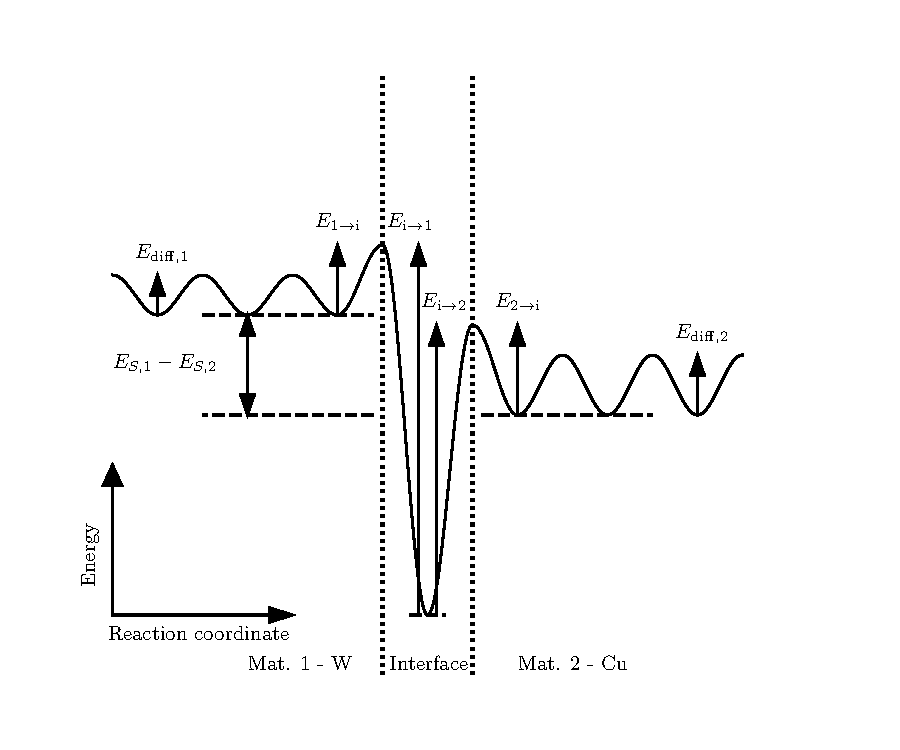
\includegraphics[width=\linewidth]{Figures/appendix/interface_E.pdf}
    \caption{Idealised potential energy diagram describing the interactions of H at the interface between two materials. In this case, $E_\mathrm{S,1}>E_\mathrm{S,2}$ (consistent with a W/Cu interface \reftab{materials properties monoblock}).}
    \label{fig:diagram_E}
\end{figure}
The interface coverage is defined as: $\theta_\mathrm{i}=\frac{c_\mathrm{i}}{n_\mathrm{i}}$ where $n_\mathrm{i}$ is the sites concentration on the interface (in \si{m^{-2}}).
% In practice, there should also be maximum concentration of sites for interstitial H ($n_{k\in\lbrace 1,2 \rbrace}$ in \si{m^{-3}}) but the concentration of interstitial H is assumed to be low compared to this maximum value, $c_k \ll n_k$: there are always a free interstitial site to detrap from the interface.
The interface is considered as a 2D defect (like a surface), hence the unit of $c_\mathrm{i}$ and $n_\mathrm{i}$ is \si{m^{-2}}.
\indent In this model, 2 types of reactions are considered at the interface:
\begin{itemize}
    \item the trapping from material $k$ to the interface: $\mathrm{H}_k \rightarrow \mathrm{H_i}$.
    \item the detrapping from the interface to material $k$: $\mathrm{H_i} \rightarrow \mathrm{H}_k$.
\end{itemize}
The rate (\si{s^{-1}}) of each reaction $x\rightarrow y$ is written with an Arrhenius law: 
\begin{equation}
\nu_{x\rightarrow y}(T)=\nu_0^{x\rightarrow y}\exp\left(-\frac{E_{x\rightarrow y}}{k_\mathrm{B}T}\right)
\label{eq:TST}
\end{equation}
with $\nu_0^{x\rightarrow y}$ (\si{s^{-1}}) the pre-exponential factor, $E_{x\rightarrow y}$ (\si{eV}) the energy barrier for the reaction $x\rightarrow y$, $k_\mathrm{B}$ (\si{eV.K^{-1}}) the Boltzmann constant and $T$ (\si{K}) the temperature.

% \indent The model outputs the the temporal evolution of the concentration of H at the interface and in the materials at the position $x_\mathrm{i}$ of the interface.
\indent The jump from interstitial site to interstitial site in material $k$ is assumed to be described by the Fick's law on diffusion characterised by the diffusion coefficient of H in material $k$ $D_{k\in\lbrace 1,2\rbrace}$ (\si{m^{2}.s^{-1}}).
Thus, the flux balance at the interface gives:
\begin{align}
\lambda_1 \left( \frac{\partial c_1}{\partial t} \right)_{x_\mathrm{i}}
                      &= \nu_{\mathrm{i}\rightarrow 1}c_\mathrm{i}
                        -\lambda_1 c_1(1-\theta_\mathrm{i})\nu_{1\rightarrow\mathrm{i}}  \nonumber
                        \\&-D_1\left(\frac{\partial c_1}{\partial x}\right)_{x_\mathrm{i}}
                        \label{eq:c1}
                        \\
\frac{d c_\mathrm{i}}{d t} 
                     &= \lambda_1 c_1 (1-\theta_\mathrm{i})\nu_{1\rightarrow\mathrm{i}}
                       - \nu_{i\rightarrow 1}c_\mathrm{i} \nonumber
                       \\ &+\lambda_2 c_2 (1-\theta_\mathrm{i})\nu_{2\rightarrow\mathrm{i}}
                       - \nu_{i\rightarrow 2}c_\mathrm{i}
                       \label{eq:ci}
                       \\
\lambda_2 \left( \frac{\partial c_2}{\partial t}\right)_{x_\mathrm{i}}
                    &= \nu_{\mathrm{i}\rightarrow 2}c_\mathrm{i}
                      -\lambda_2 c_2 (1-\theta_\mathrm{i})\nu_{2\rightarrow\mathrm{i}} \nonumber
                      \\ &+D_2 \left(\frac{\partial c_2}{\partial x}\right)_{x_\mathrm{i}}
                      \label{eq:c2}
\end{align}
where $\lambda_{k\in\lbrace 1,2 \rbrace}$ (\si{m}) is the distance between two interstitial sites in material $k$ (such that $\lambda_k c_k(x_\mathrm{i})$ represent the areal density of interstitial H at the depth $x_\mathrm{i}$ which interacts with the interface).
In Equations~\ref{eq:c1} and~\ref{eq:c2}, the first term on the right-hand side corresponds to the detrapping from the interface to material $k$, the second term correspond to the trapping to the interface and the last term corresponds to the diffusion that carries away particles from the interface region (it is important to note that the signs of these fluxes are different).
\indent At steady-state, when the time derivatives are null and the diffusive flux can be neglected (i.e.\ when the diffusion depth is long compared to $\lambda_k$), one gets:
\begin{equation}
     \frac{c_2}{c_1}=\frac{\lambda_1}{\lambda_2}\frac{\nu_\mathrm{i\rightarrow2}(T)}{\nu_\mathrm{2\rightarrow i}(T)}\frac{\nu_\mathrm{1\rightarrow i}(T)}{\nu_\mathrm{i\rightarrow 1}(T)} = \frac{S_2(T)}{S_1(T)}
\end{equation}
% Replacing each $\nu_{x\rightarrow y}(T)$ by the Arrhenius law (equation~\ref{eq:TST}), it leads to:
%\begin{equation}
%    \frac{c_2}{S_2}=\frac{c_1}{S_1}
%\end{equation}
with $S_k(T)$ (\si{m^{-3}.Pa^{-0.5}}) the solubility of H in material $k$.
The condition to have such steady-state is:
\begin{equation}
    E_{S,1}-E_{S,2} = E_\mathrm{i\rightarrow 1}-E_\mathrm{i\rightarrow 2}-E_\mathrm{1\rightarrow i} +E_\mathrm{2\rightarrow i}
    \label{eq:steady}
\end{equation}
% This is equivalent to Equation~\refeq{c/s conservation} used in this study.

% \section{Test case}
\indent The simple kinetic presented here allows us to see how fast the equilibrium given by \refeq{c/s conservation} is reached.
% If it is much faster than the characteristic time of the simulation presented in section~\ref{iter case}, one can consider that the use of such kinetic model is of now use for as it would not significantly affect the dynamic of permeation for the considered thickness.
For the test case, we further simplify the model by considering that the concentration of interstitial H in material 1 $c_1$ is constant (\textit{ie.} $\partial c_1/\partial t=0$).
The diffusive fluxes are neglected in Equation~\ref{eq:c2} in order to solve a 0D problem.
The system of equation is solved with the SciPy package~\cite{virtanen_scipy_2020} which uses the odepack library~\cite{hindmarch_odepack_1982}.
% \indent As for the trapping around defects, we consider that the activation energy for the trapping reaction to the interface from material $k$ is the energy barrier for the diffusion $E_{k\rightarrow\mathrm{i}}=E_{\mathrm{diff},k}$.
% In addition, we consider that all the pre-exponential factor are equal to 10$^{13}$ \si{s^{-1}}.
% It means that, in order to have the steady-state equation (equation~\ref{eq:steady}) equivalent to \refeq{c/s conservation}, one needs $\frac{S_{0,1}}{S_{0,2}}=\frac{\lambda_2}{\lambda_1}$.
% Fixing all these parameters, the only free parameters are the detrapping energy from the interface to the materials. 

% Again, to satisfy the steady-state condition, one needs:
% \begin{equation}
%     E_{S,1}-E_{S,2} = E_\mathrm{i\rightarrow 1}-E_\mathrm{i\rightarrow 2}-(E_\mathrm{1\rightarrow i}-E_\mathrm{2\rightarrow i})
% \end{equation}


% Since, we already fixed the value of $E_{\mathrm{i\rightarrow},k}$ to the diffusion barrier in material $k$ and since $E_{S,1}-E_{S,2}$ is fixed for a set of materials, there is actually only one free parameter.
\indent A W/Cu interface is simulated at \SI{475}{K}.
% We fix the concentration of H in tungsten to $c_1=10^{18}$ \si{m^{-3}}.
% The trapping energy to the interface are 0.39 eV for both materials (table~\ref{tab:materials properties}).
% For W, we consider $\lambda_1=110$ pm.
% Thus, as discussed in the previous paragraph, it fixes $\lambda_2=65$ pm.
All parameters in the model have been constrained so that it corresponds to the steady state condition in equation~\ref{eq:steady} in the case of a W/Cu interface considering for both W and Cu, $E_{k\rightarrow i}=E_{\mathrm{diff},k}$ with $k$=Cu or W.
The values of $\lambda$ for W and Cu are \SI{110}{pm} and \SI{65}{pm} respectively.
The concentration of H in W is set to $c_1=\SI{e18}{m^{-3}}$.
The concentration of trapping site at the interface is set to $n_\mathrm{i}=10^{19}$ \si{m^{-2}}.
All pre-exponential factors are set to \SI{e13}{s^{-1}}.
% No value for the detrapping energy from the W/Cu are known so far, so we consider $0.53 \ \mathrm{eV} \le E_\mathrm{i \rightarrow 2} \le  1.13 \ \mathrm{eV}$ which means that $1.00 \ \mathrm{eV} \le E_\mathrm{i \rightarrow 1} \le 1.60 \ \mathrm{eV}$.
The only free parameter left is $E_{\mathrm{i\rightarrow},2}$ and a parametric study is performed (see Figure~\ref{fig:kinetic_interface}).
% for the various values of $E_\mathrm{i\rightarrow 2}$: (a) the evolution of the concentration in material 2 with the normalised time $t/\tau_2$, (b) the evolution of interface coverage with the normalised time $t/\tau_\mathrm{i}$, (c) the evolution of $\tau_\mathrm{i}$ and $\tau_2$ and (d) of the interface coverage at steady-state with the detrapping energy from the interface to the material 2.

The ratio $c_2/c_1$ steady state value is approximately $10^5$ (see Figure~\ref{fig:kinetic_interface}(a)).
The ratio $\theta_\mathrm{i}/\theta_\mathrm{i}^\mathrm{eq}$ does not depend on the value of the detrapping energy (see Figure~\ref{fig:kinetic_interface}(b)).
$\tau_\mathrm{i}$ and $\tau_2$ are defined as the time at which $c_\mathrm{i}$ and $c_2$ have reached 95\% of their equilibrium value.
In this case, both $\tau_\mathrm{i}$ and $\tau_2$ remain below \SI{e3}{s} (see Figure \ref{fig:kinetic_interface}(c)).
The interface is saturated with H for $E_{\mathrm{i\rightarrow},2}/(k_B T) > 25$ (see Figure \ref{fig:kinetic_interface}(d)).
% However, the equilibrium concentration strongly depends on the value of $E_\mathrm{i\rightarrow 2}$: at 475 K, the interface is saturated with H above 1 eV while the coverage is below $10^{-4}$ for 0.53 eV (figure~\ref{fig:kinetic_interface}(d)).
% The evolution of $c_2/c_1$ does not depend on the value of $E_\mathrm{i\rightarrow2}$ only in the range 0.53 - 0.88 eV (figure~\ref{fig:kinetic_interface}(a)): at 475 K, the kinetic processes are fast with such energies and the value of $\tau_\mathrm{i}$ and $\tau_2$ are identical (figure~\ref{fig:kinetic_interface}(c)).
% However, above 0.88 eV, $\tau_\mathrm{i}<\tau_2$ and one can see a delay of the growth of $c_2/c_1$: as $\theta_\mathrm{i}^\mathrm{eq}$ is much higher, one needs to wait a longer time to first fill the interface and then transfer H from the interface to material 2 efficiently.
% Regarding the value of the characteristic time $\tau_\mathrm{i}$ and $\tau_2$, they are all below 1000 s for the considered range of detrapping energies: compared to the simulation of ~10$^7$ seconds, the equilibrium at the interface can be considered to be reached much faster than the growth of the inventory and the permeation flux (see section~\ref{bi-material} and section~\ref{iter case}).
% The only difference, is that the total tritium inventory lacks the amount retained in the interface which can be significant for the highest detrapping energies.
% No knowledge of detrapping energies are know so far for the W/Cu interface.
% However, the case $E_\mathrm{i\rightarrow2}=1.13$ eV corresponds to $E_\mathrm{i\rightarrow1}=1.60$ eV.
% In tungsten, a trap with a detrapping energy of 1.6 eV is a quite a deep trap such as monovacancy~\cite{fernandez_hydrogen_2015} or small vacancy cluster~\cite{pecovnik_new_2020, hou_predictive_2019}.
% If one considers that traps at the interface are as deep as trap in the materials (0.57 eV in table~\ref{tab:materials properties}), the characteristic time are very small (0.1 s) and the retention at the interface is negligible ($10^{15}$ m$^{-2}$) making \refeq{c/s conservation} a good approximation for the estimation of very macroscopic retention and permeation properties of the ITER monobloc.

\begin{figure} [h!]
    \centering
    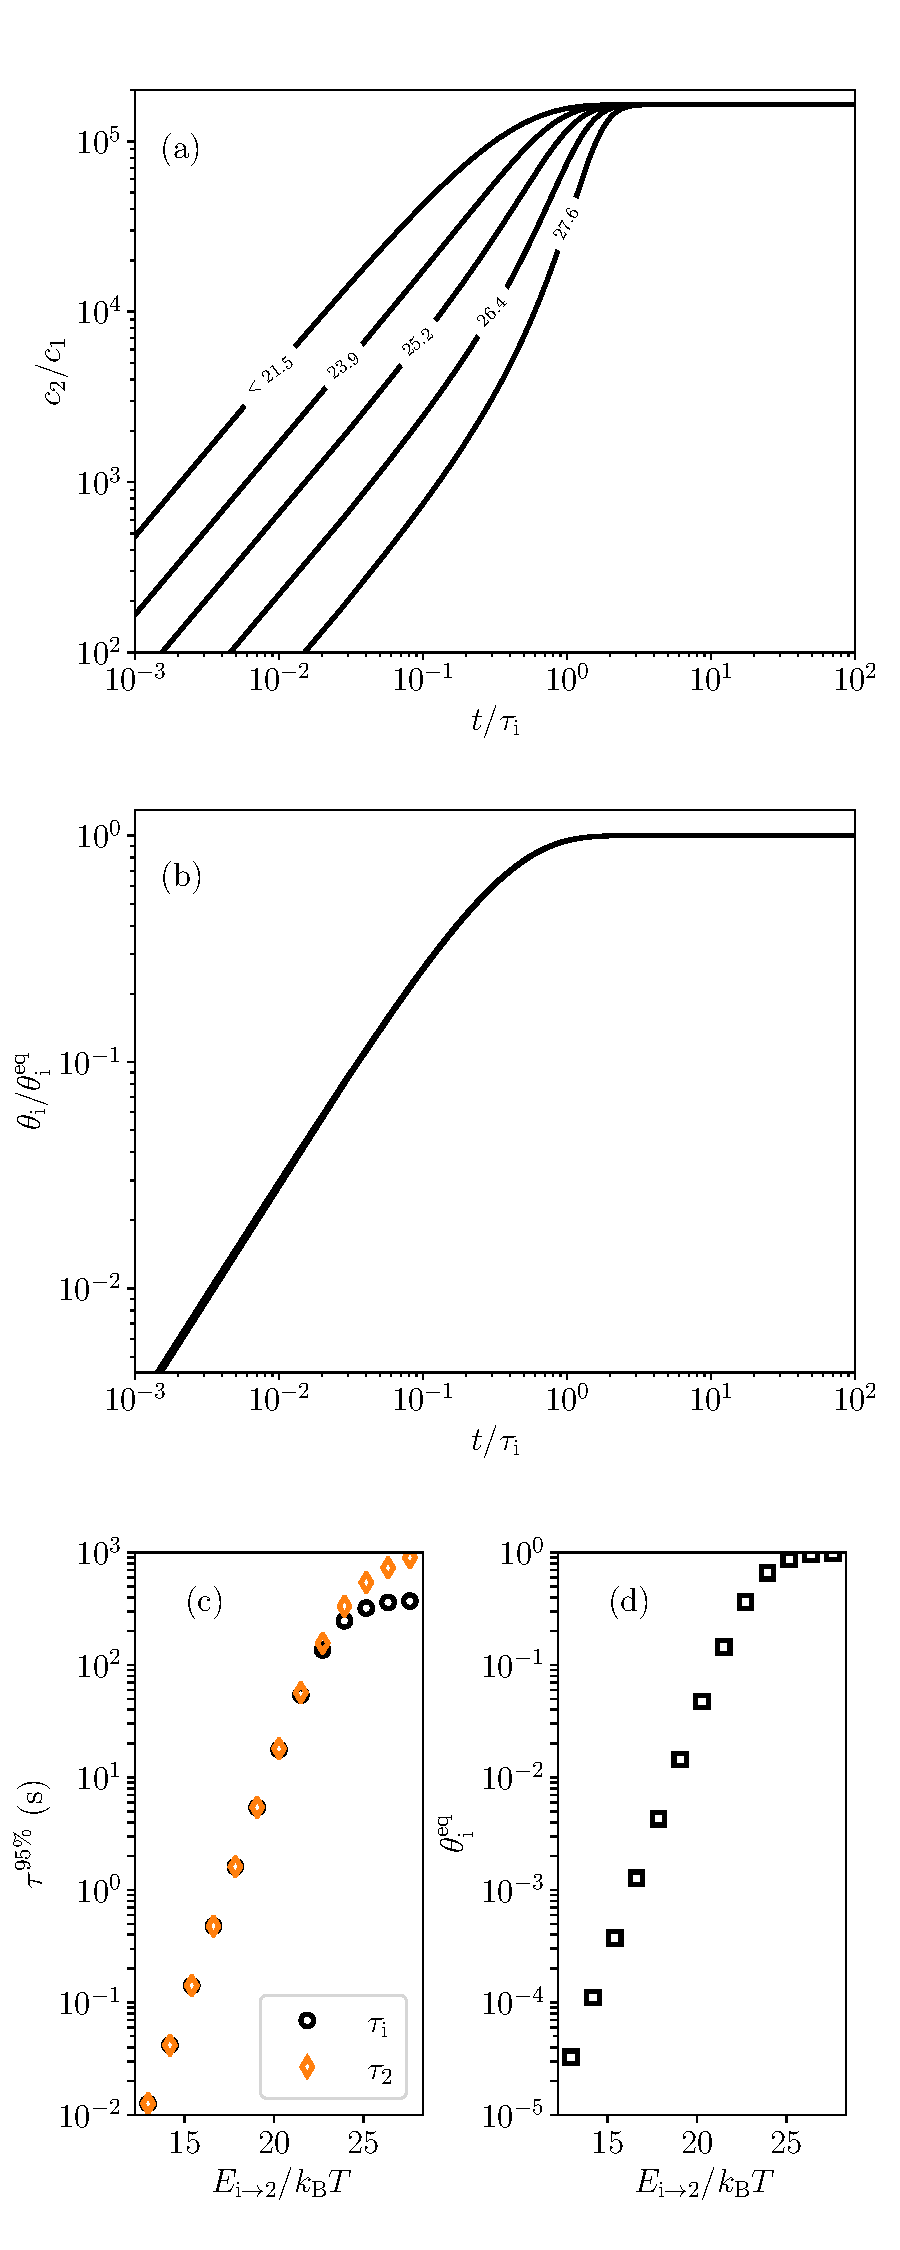
\includegraphics[width=0.8\linewidth]{Figures/appendix/kinetic_interface.pdf}
    \caption{(a) Evolution of the ratio $c_2/c_1$ with normalised time $t/\tau_\mathrm{i}$ for different values of $E_\mathrm{i \rightarrow 2}/k_\mathrm{B}T$.
    (b) Evolution of the ratio $\theta_\mathrm{i}/\theta_\mathrm{i}^\mathrm{eq}$ with normalised time $t/\tau_\mathrm{i}$ (independent of $E_\mathrm{i\rightarrow2}/k_\mathrm{B}T$).
    (c) Evolution of the time to reach 95\% of the steady-state concentration, $\tau_\mathrm{i}$ and $\tau_\mathrm{2}$ as a function of $E_\mathrm{i \rightarrow 2}/k_\mathrm{B}T$.
    (d) Evolution of $\theta_\mathrm{i}^\mathrm{eq}$ as a function of $E_\mathrm{i\rightarrow2}/k_\mathrm{B}T$.
    The temperature in the simulation is 475 K, the concentration in the material 1 (W) is $c_1=10^{18}$ \si{m^{-3}} and the concentration of trapping site at the interface is $n_\mathrm{i}=10^{19}$ \si{m^{-2}}.}
    \label{fig:kinetic_interface}
\end{figure}

